\newpage
{\samepage
\begin{center}
{\Large{\bf Hashing}}
\end{center}
\begin{itemize}
\item To keep records of employees we might index (search) them by using
their National Insurance number: \verb^xx-##-##-##-x^
\item There are $17.6$ billion combinations (around $2^{34}$).
\item Could use an array of $17.6$ billion entries, which would make searching
for a particular entry trivial !
\item Especially wasteful since only our ($5000$) employees need to be
stored.
\item In this lecture we examine a method that, using an array of $6000$
elements, would require $2.1$ comparisons on average.
\end{itemize}
}

\newpage
{\samepage
\begin{center}
{\Large{\bf Hashing Nomenclature}}
\end{center}
{\small
\begin{itemize}
\item A hash function is a mapping, h(K), that maps from key K, onto the index of an entry.
\item A black-box into which we insert a key (e.g. NI number) and out pops an array index.
\item As an example lets use an array of size $11$ to store some airport codes, e.g.
\verb^PHL^, \verb^DCA^, \verb^FRA^.
\item In a three letter string $X_2 X_1 X_0$ the letter 'A' has the value 0, 'B' has the
value 1 etc.
\item One hash function is:
\[
h(K) = (X_2*26^2 + X_1*26 + X_0)\%11
\]
\item Applying this to "DCA":\\

$ h("DCA") = (3*26^2 + 2*26 + 0)\%11$\\

$ h("DCA") = (2080)\%11$\\

$ h("DCA") = 1 $
\end{itemize}
}}

\newpage
{\samepage
\begin{center}
{\Large{\bf Collisions}}
\end{center}
\begin{itemize}
\item Inserting "PHL", "ORY" and "GCM":
\begin{center}
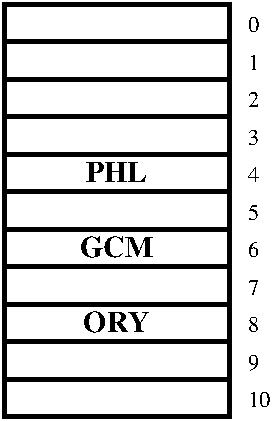
\includegraphics{../Images/hashapt.pdf}
\end{center}
\item However, inserting "HKG" causes a collision.
\begin{center}
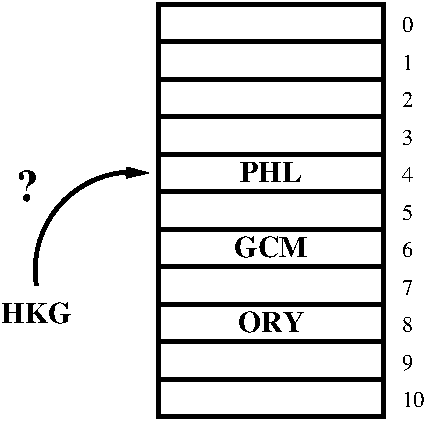
\includegraphics{../Images/hashclash.pdf}
\end{center}
\end{itemize}
}

\newpage
{\samepage
\begin{center}
{\Large{\bf Collisions}}
\end{center}
\begin{itemize}
\item An ideal hashing function maps keys into the array in a {\it uniform} and {\it random} manner.
\item Collisions occur when a hash function maps two different keys onto the same address.
\item It's very difficult to choose 'good' hashing functions.
\item Collisions are common - the {\bf von Mises} paradox. When 23 keys are randomly mapped onto 365 addresses there is a 50\% chance of a collision.
\end{itemize}
}

\newpage
{\samepage
\begin{center}
{\Large{\bf Linear Probing}}
\end{center}
{\small
\begin{center}
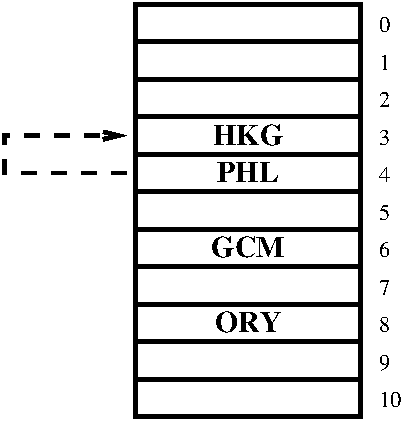
\includegraphics{../Images/hashprobe.pdf}
\begin{itemize}
\item The policy of finding another free location if a collision occurs is called open-addressing.
\item If a collision occurs then keep stepping backwards (with wrap-around) until a free location is encountered.
\item The simplest method of open-addressing is linear-probing.
\item The step taken each time (probe decrement) need not be~1.
\item Open-addressing through use of linear-probing is a very simple technique, double-hashing is generally much more successful.
\end{itemize}
\end{center}
}}

\newpage
{\samepage
\begin{center}
{\Large{\bf Double Hashing}}
\end{center}
\begin{itemize}
\item A second function p(K) decides the size of the probe decrement.
\item The function is chosen so that two keys which collide at the same address will have different probe decrements, e.g. :
{\small
\[
p(K) = MAX (1, ((X_2*26^2 + X_1*26+X_0)/11)\%11)
\]
}
\item Although "PHL" and "HKG" share the same primary hash value of $h(K)=4$, they
have different probe decrements:

$p("PHL")=4$\\

$p("HKG")=3$
\end{itemize}
}

\newpage
{\samepage
\begin{center}
{\Large{\bf Prime Array Sizes}}
\end{center}
\begin{itemize}
\item If the size of our array, $M$, was even and the probe decrement was chosen to be $2$, then only half of the locations could be probed.
\begin{center}
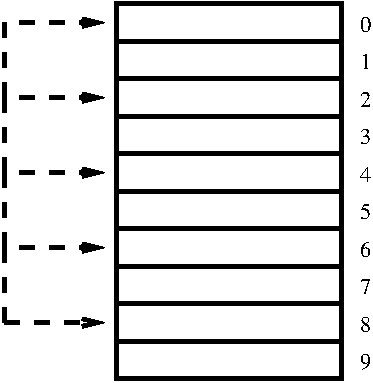
\includegraphics{../Images/hashp2.pdf}
\end{center}
\item Often we choose our table size to be a prime number and our probe decrement to be a number in the range $1 \ldots M-1$.
\end{itemize}
}

\newpage
{\samepage
\begin{center}
{\Large{\bf Separate Chaining}}
\end{center}
Open-addressing is not the only method of collision reduction. Another common
one is separate chaining.
\begin{center}
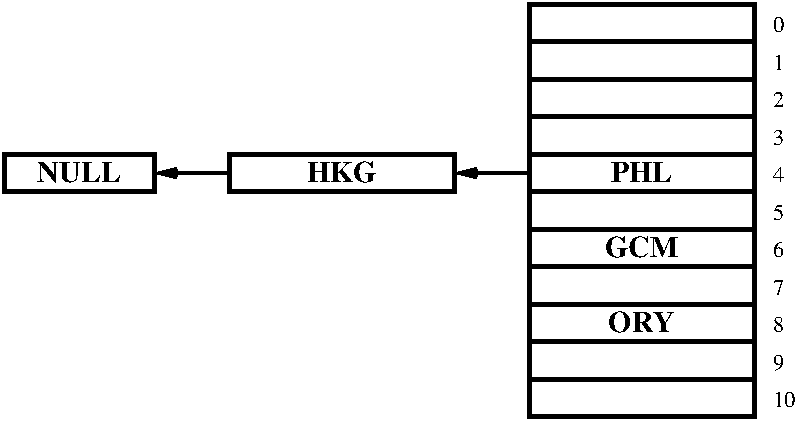
\includegraphics{../Images/hashsep.pdf}
\end{center}
}

\newpage
{\small
\begin{verbatim}
/*
Modified Bernstein hashing
5381 & 33 are magic numbers required by the algorithm
*/
int hash(unsigned int sz, char *s)
{
   unsigned long hash = 5381;
   int c;
   while((c = (*s++))){
      hash = 33 * hash ^ c;
   }
   return (int)(hash%sz);
}
\end{verbatim}

Has many similarities to the implementation of the pseudo-random number generator in C, \verb^rand()^.
{\small
\begin{verbatim}
/* This algorithm is mentioned in the ISO
   C standard, here extended for 32 bits. */
int rand_r (unsigned int *seed)
{
  unsigned int next = *seed;
  int result;
  next *= 1103515245;
  next += 12345;
  result = (unsigned int) (next / 65536) % 2048;
  ... ETC ...
\end{verbatim}
}
}

\newpage
{\samepage
\begin{center}
{\Large{\bf Cuckoo Hashing}}
\end{center}
{\tiny
\begin{verbatim}
Empty: copied farandoles into table 0(4)
Empty: copied bronzine into table 0(12)
Empty: copied auscultatory into table 0(5)
Empty: copied bifer into table 0(13)
Empty: copied steepgrass into table 0(6)
Empty: copied prevised into table 0(7)
Empty: copied oomph into table 0(8)
empodium, so cuckooed out auscultatory from table 0(5)
Empty: copied auscultatory into table 1(10)
interquarreled, so cuckooed out bronzine from table 0(12)
Empty: copied bronzine into table 1(5)
ranseur, so cuckooed out empodium from table 0(5)
Empty: copied empodium into table 1(4)
Empty: copied megalodon into table 0(11)
geosynchronous, so cuckooed out megalodon from table 0(11)
Empty: copied megalodon into table 1(14)
Empty: copied osmeteria into table 0(14)
Table getting full -> rehashed old sz =16
\end{verbatim}
}
\vspace*{-0.5in}
\begin{center}
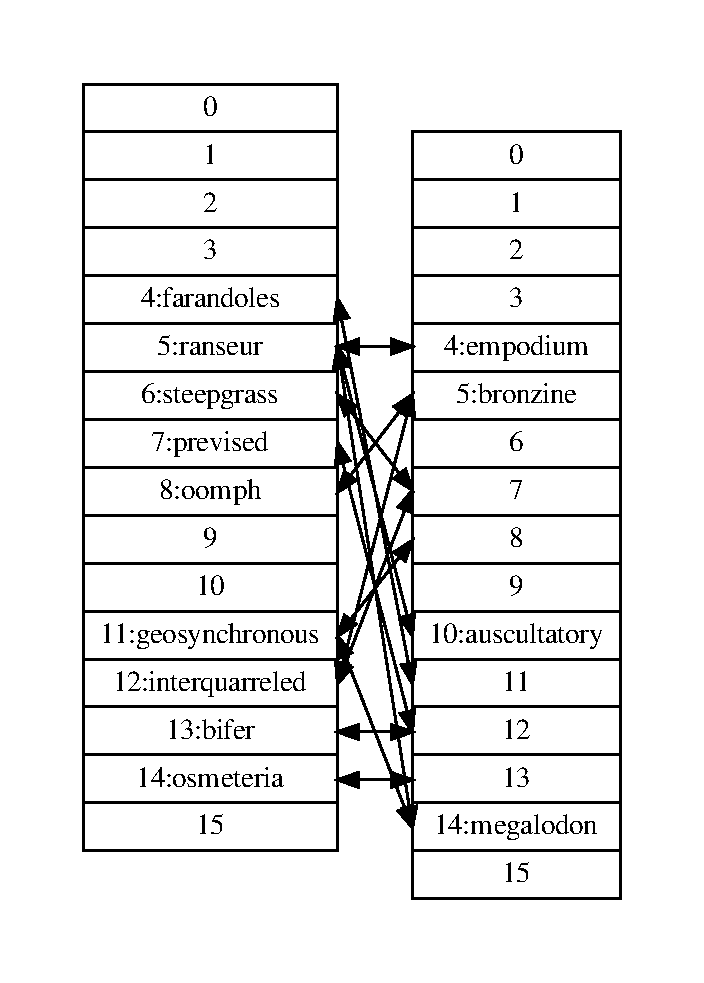
\includegraphics[scale=1.00]{../Images/cuckoo.pdf}
\end{center}
}
